\documentclass[10pt,a4paper]{amsart}
\usepackage[margin=19mm]{geometry}
\usepackage{amsmath,amssymb,mathtools}
\usepackage[scr=rsfs,cal=euler]{mathalfa}
\usepackage{xfrac}
\usepackage[unicode,hidelinks,bookmarks=false]{hyperref}
\newcommand{\ie}{i.e.\ }
\newcommand{\cf}{cf.\ }
\newcommand{\resp}{respectively\ }
\newcommand{\Subsection}{\subsection}
\providecommand{\nobreakdash}{\nobreak\hbox{-}}
\setlength{\emergencystretch}{2em}
\multlinegap0pt
\usepackage{tikz}
\usepackage{amssymb}
\usepackage{xcolor}
\usepackage[normalem]{ulem}
\usepackage{mathtools}
\newtheorem{remark}{Remark}
\newtheorem{lemma}{Lemma}
\newtheorem{corollary}{Corollary}
\newtheorem{proposition}{Proposition}
\newcommand{\EE}{\mathbb E}
\newcommand{\RR}{\mathbb R}
\newcommand{\cE}{\mathcal E}
\newcommand{\one}{{\bf 1}\hskip-.5mm} %\def\one{{\bf 1}\hskip-.5mm}
\newcommand{\sM}{\mathsf{M}}
\newcommand{\sN}{\mathsf{N}}
\newcommand{\se}{{\mathsf{e}}}
\newcommand{\ua}{\underline a}
\newcommand{\ub}{\underline b}
\newcommand{\uell}{\underline \ell}
\newcommand{\uu}{\underline u}
\newcommand{\vep}{\varepsilon}
\title{\textsc{Slot decomposition of\\ continuous Box-Ball Systems}}
\author{In\'es Armend\'ariz, Pablo Blanc, Pablo A. Ferrari, Davide Gabrielli}
\date{Source: arXiv:2606.20948v1 (CC BY 4.0)}
\begin{document}
\maketitle

\noindent\emph{Source and licence.} \textsc{Slot decomposition of\\ continuous Box-Ball Systems}. Version arXiv:2606.20948v1 (CC BY 4.0), distributed by arXiv under the Creative Commons Attribution 4.0 International licence, http://creativecommons.org/licenses/by/4.0/, as recorded in the arXiv licence metadata for this exact version and shown on the abstract page https://arxiv.org/abs/2606.20948v1. Full licence notice: \texttt{licenses/arxiv-2606.20948-CC-BY-4.0.txt}.\par\smallskip

\noindent\textit{Editorial scope.} Counted unit: the article's proposition eqm9 (source0.tex lines 1633--1638). The article's complete original proof of it is delivered with it (source0.tex lines 1639--1714, one \texttt{proof} environment of 76 lines). No mathematics is written, repaired or re-derived: the statement and the proof are the article's own lines, in the article's own notation, and no retained line is substituted or re-flowed.  Retained uncounted as the source-local context the proof needs: lines 1355--1359; lines 1361--1364; lines 1428--1433; lines 1489--1493; lines 1533--1535; lines 1596--1601; lines 1609--1612; lines 1619--1626.  Nothing was omitted from any retained span, so the package carries no omission record.  No retained line contains a citation, so the wrapper carries no bibliography and no bibliography entry.  The retained lines contain the article's own diagram code, which the wrapper typesets with the standard tikz packages; no image file is delivered and the package declares no asset dependency.  Editorial formatting only, in addition: an AMS \texttt{amsart} preamble that restates the article's own declarations and macros used by the retained lines, namely the environments \texttt{remark}, \texttt{lemma}, \texttt{corollary}, \texttt{proposition} on separate counters, together with the standard packages those lines need.  The retained environments print in this document as Remark 1, Lemma 1, Corollary 1, Proposition 1 in order of appearance, whereas the article prints the same items with the numbering of its own full document.  The complete native source of the article as distributed in the arXiv e-print for this exact version is bundled unchanged as \texttt{sources/203249/source0.tex}.
\begin{align}
	\label{mua1}
	\mu_\alpha(d\varepsilon)
  &\vcentcolon =\frac{1}{Z_\alpha}\, \sum_{n=1}^\infty\one\{\vep\in\cE_o(n)\}\, \alpha(\ell_1)\dots\alpha(\ell_n)\, d\ua_n\, d\ub_{n}\,.
    \end{align}

\begin{equation}
	\label{mua2}
	\mathcal A^+\vcentcolon =\Bigl\{\alpha\,:\,\int \se(\varepsilon)\,\mu_\alpha(d\varepsilon)< +\infty\Bigr\}\,
\end{equation}

\begin{remark}(Law of the excursion maximum)\label{maxi}
The maximum value $\ell_1$ of the excursion $\sM$ has distribution
\begin{equation}\label{maxlaw}
 \frac{q(\ell)\,d\ell}{\int_0^{+\infty} q(\ell)d\ell}.
\end{equation}
\end{remark}

\begin{align}
	\label{nuq5}
	\nu_q(d\uu_n\, d\uell_n) &= \frac{\one_{\mathcal N_o}\left(\underline u_n, \underline \ell_n\right)}{\int q(y)dy}\, \prod_{i=1}^n \exp\Bigl(-2\int_0^{\ell_i} (\ell_i-y)\, q(y)\, dy\Bigr)\, q(\ell_i)\, d\uu_n\, d\uell_n \notag\\
	&= \frac{\one_{\mathcal N_o}\left(\underline u_n, \underline \ell_n\right)}{\int q(y)dy}\, \prod_{i=1}^n \exp\big(-2\mathcal Q(\ell_i)\big)\, \mathcal Q''(\ell_i)\, d\uu_n\, d\uell_n ,
\end{align}

\begin{lemma}[Finite slot diagrams]\label{Tpos}
Let $\sN$ be a Poisson point process on $\RR\times \RR_+$ with intensity measure $du\,q(\ell) d\ell$, and let $\sM$ be the leftmost slot diagram in $\sN_+$. Then $\sM$ contains a finite number of points with probability $1$.
\end{lemma}

\begin{corollary}[Finite mean excursion length]\label{mlength}
Let $q\in \mathscr Q$. Consider the Poisson point process $\sN$ in $\RR\times \RR_+$ with intensity $du\, q(\ell)d\ell$, and let $\sM$ be the leftmost excursion of $\sN_+$. Then its mean length
\begin{align}\label{3133}
\EE\big[ \sum_{(u_i,\ell_i) \in \sM}2\ell_i\big]=\frac{\int_0^\infty m(\ell) q(\ell) d\ell}{\int_0^\infty q(\ell) d\ell}<+\infty \iff q\in \mathscr Q^+.
\end{align}
\end{corollary}

	\begin{align}
		\label{a=q}
		\alpha(\ell) \vcentcolon= q(\ell)\, \exp\Bigl(-2\int_0^\ell(\ell-y)\, q(y)\, dy\Bigr)\,, \qquad \ell\in \mathbb R^+\,.
	\end{align}

	\begin{equation}\label{lequazione1}
		\left\{
		\begin{array}{l}
			\mathcal Q''(y)=\alpha(y) e^{2\mathcal Q(y)}, \\
			\mathcal Q(0)=\mathcal Q'(0)=0,
		\end{array}
		\right.
	\end{equation}

\begin{proposition}[Equivalence of measures]
	\label{eqm9}
	Consider the relation  between the functions $\alpha$ and $q$ given by equations \eqref{a=q} and the Cauchy problem \eqref{lequazione1}.
	This defines a bijection between $\mathcal A$ and $\mathscr Q$ and between $\mathcal A^+$ and $\mathscr Q^+$. Moreover if $\alpha$ and $q$ are in bijection then 
	$ \mu_\alpha=\nu_q$ and $Z(\alpha)=\int_{\RR_+} q(\ell)\, d\ell$.
\end{proposition}

\begin{proof}
	
	
	We first show that for each fixed $n$,
the variables $(\underline u_n,\underline \ell_n)$ and $(\underline a_n,\underline b_n)$
are related by a volume preserving linear transformation, i.e. we show that the Jacobian determinant of this transformation is $1$. 

We proceed by induction. First of all the Jacobian determinant of the transformation is one when $n=1$ since in that case there are just the variables $\ell_1$ and $b_1$ with $\ell_1=b_1$. We assume that the statement is true for $n$ and show that it is then true for $n+1$. 

Consider an excursion having $n$ solitons with lengths $\ell_1\geq \ell_2\geq \dots \geq \ell_{n}$. Let us call $(\underline u_n,\underline \ell_n)$ the coordinates in the first representation, and let $(\underline a_n, \underline b_n)$be  the corresponding variables in the other coordinate system. By inductive hypothesis we have
$(\underline a_n, \underline b_n)=A(\underline u_n, \underline \ell_n)$ where $A$ is a $(2n-1)\times (2n-1)$ matrix 
having $|A|=\pm 1$. Indeed the structure of the matrix $A$ changes for different regions of the parameters but not the value of the determinant.
We call $(A_{i,j})_{1\leq i,j\leq 2n-1}$ the elements of the matrix $A$.

In Fig.~\ref{transform} we present an excursion with $n=3$ red solitons to which we attach a new blue soliton. After attaching this soliton of length $\ell_{n+1}\leq \ell_n$, the updated coordinates become
$(\underline u_n, \underline \ell_n, u_{n+1}, \ell_{n+1})$. 
The slot diagram of the new excursion will be in correspondence with coordinates $(\tilde{\underline a}_n, \tilde{\underline b}_n, a', b')$, where $(a',b')$ are the coordinates respectively of the new minimum and maximum created by the insertion of the soliton. Here $(\tilde{\underline a}_n,\tilde{\underline b}_n)$ denote the coordinates of the local minima and maxima that were present before the insertion of the soliton, and whose position may have changed due to the new addition. 
\begin{figure}
	
	\centering
	
	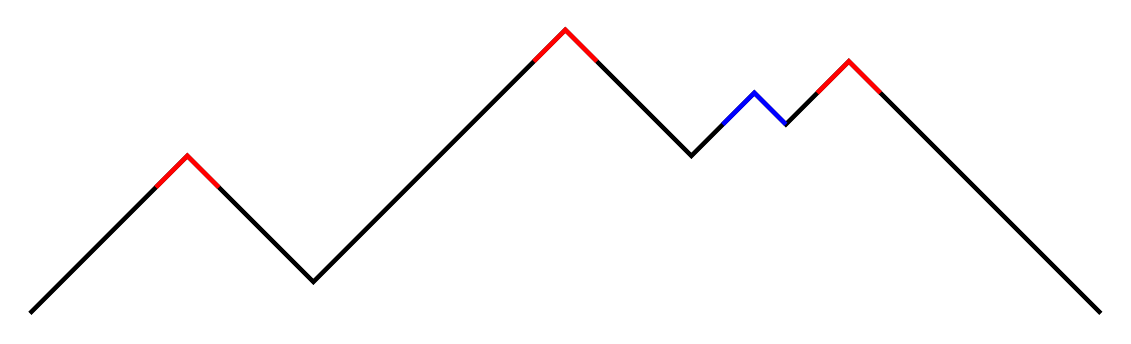
\begin{tikzpicture}[scale=0.4, thick]

    
    
    \draw[ultra thick] (0,0) -- (5,5) -- (9,1) -- (17,9) -- (21,5) -- (23,7)-- (24,6)-- (26,8) -- (34,0);
    
    
    \draw[blue, ultra thick] (22,6) -- (23,7) -- (24,6);
    
    \draw[red, ultra thick] (4,4) -- (5,5) -- (6,4);
    \draw[red, ultra thick] (16,8) -- (17,9) -- (18,8);
    \draw[red, ultra thick] (25,7) -- (26,8) -- (27,7);

\end{tikzpicture}
	
	\caption{We attached the new smallest blue soliton; the dark part of the excursion is the slot space where it is possible to attach the soliton, the red part where it is not possible. }
	
	\label{transform}
\end{figure}

Suppose we insert the $(n+1)$-th soliton following the first $k$ maxima, and let us assume that it is attached in the left part of a soliton, so that the coordinate of the new local maximum $b'$ is smaller than the coordinate of the new local minimum $a'$.
This corresponds to the case shown in Fig.~\ref{transform} with $k=2$. The other case ($a'<b'$) can be handled in a similar way.

We have that $\tilde a_i=a_i$ and $\tilde b_i=b_i$ for $i=1,\dots , k$ so that in particular these coordinates do not depend on the variables $(u_{n+1},\ell_{n+1})$. We have moreover $b'=u_{n+1}+(2k+1)\ell_{n+1}$ and $a'=u_{n+1}+(2k+2)\ell_{n+1}$
and finally $\tilde b_i=b_i+2\ell_{n+1}$ and $\tilde a_i=a_i+2\ell_{n+1}$ for $i=k+1,\dots , n$. Therefore the matrix for the change of variables form $(\underline u_n,\underline \ell_n, u_{n+1}, \ell_{n+1})$ to $(\tilde{\underline a}_n, \tilde{\underline b}_n, a',b')$ is given as follows
\[
\left(\begin{matrix}
	A_{11}& \dots & A_{1,2n-1} & 0 & 0 \\
	\vdots & \vdots & \vdots & \vdots & \vdots \\
	A_{k-1,1} & \dots & A_{k-1,2n-1} & 0 & 0 \\
	A_{k,1} & \dots & A_{k,2n-1} & 0 & 2\\
	\vdots & \vdots & \vdots & \vdots & \vdots \\
	A_{n-1,1} & \dots & A_{n-1,2n-1} & 0 & 2 \\
	A_{n,1} & \dots & A_{n,2n-1} & 0 & 0\\
	\vdots & \vdots & \vdots & \vdots & \vdots \\
	A_{n+k-1,1} & \dots & A_{n+k-1,2n-1} & 0 & 0 \\
	A_{n+k,1} & \dots & A_{n+k, 2n-1} & 0 & 2\\
	\vdots & \vdots & \vdots & \vdots & \vdots \\
	A_{2n-1,1} & \dots & A_{2n-1,2n-1} & 0 & 2 \\
	0 & \dots & 0 & 1 & 2k+2 \\
	0 & \dots & 0 & 1 &  2k+1\\
\end{matrix}\right)
\]
If we develop the determinant of the above $(2n+1)\times (2n+1)$ matrix along the second to last column we get that, up to a $\pm$ sign in front, its determinant is equal to
\[
(2k+2)|A|-(2k+1)|A|=|A|=1\,,
\]
where the last identity follows by the inductive hypothesis.	
		
Consider $q\in \mathscr Q$. By Lemma \ref{Tpos}, $\nu_q$ given in \eqref{nuq5} is a probability measure, and relation \eqref{a=q} and the fact that the Jacobian transformation has determinant $1$ imply that $\mu_{\alpha}$ in \eqref{mua1} is a probability measure as well, so that $\alpha\in \mathcal A$. Conversely, consider $\alpha\in \mathcal A$ so that $\mu_{\alpha}$ is a probability measure, and let $q$ be computed by the solution of the Cauchy problem \eqref{lequazione1}. Once again, it follows from the fact that the determinant of the Jacobian transformation is $1$ that $\nu_q$ is a probability measure. By Remark \ref{maxi} the maximum value of the excursion has law given by \eqref{maxlaw}, and hence $q\in \mathscr Q$.
	
The bijection between the sets $\mathcal A^+$ and $\mathscr Q^+$ is similarly obtained. By Corollary \ref{mlength} the average length of the leftmost excursion $\sM$ is finite if and only if 
$q\in \mathscr Q^+$. On the other hand, from \eqref{mua2}, the excursion with law $\mu_\alpha$ has finite length only when $\alpha \in \mathcal A^+$, so we conclude that $q\in \mathscr Q^+$ if and only if $\alpha \in \mathcal A^+$.

Finally, in view of expressions \eqref{mua1} and \eqref{nuq5} of the measures $\mu_\alpha$ and $\nu_q$, respectively, and relation \eqref{a=q} that defines $\alpha$ in terms of $q$, the normalizing constants $Z(\alpha)$ and $\int_0^{+\infty} q(y)dy$ must be equal. \end{proof}

\end{document}
